\documentclass[twocolumn]{IEEEtran}
\usepackage{amsmath,amssymb,amsfonts}
\usepackage[table]{xcolor}
\usepackage{tikz}
	\usepackage {xcolor}

\begin{document}

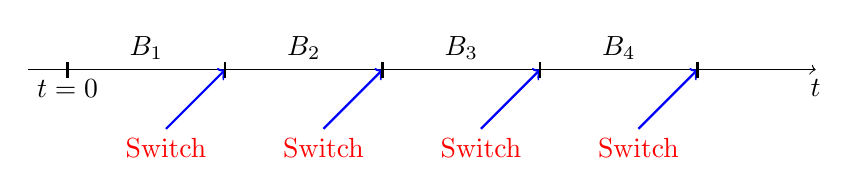
\begin{tikzpicture}
\path (0.5, 0) coordinate (A) node[below] {$t=0$};
\path (10, 0) coordinate (B) node[below] {$t$};
\draw[arrows={->[slant=.3]}]  (0,0) -- (10,0);
\draw[thick, blue, arrows={->[slant=.3]}] (1.75,-0.75)--(2.5,0);
\draw[thick, blue, arrows={->[slant=.3]}] (3.75,-0.75)--(4.5,0);
\draw[thick, blue, arrows={->[slant=.3]}] (5.75,-0.75)--(6.5,0);
\draw[thick, blue, arrows={->[slant=.3]}] (7.75,-0.75)--(8.5,0);
\draw[thick] (0.5,-0.1)--(0.5,0.1);
\draw[thick] (2.5,-0.1)--(2.5,0.1);
\draw[thick] (4.5,-0.1)--(4.5,0.1);
\draw[thick] (6.5,-0.1)--(6.5,0.1);
\draw[thick] (8.5,-0.1)--(8.5,0.1);
\path (1.5, 0) coordinate (A1) node[above] {$B_1$};
\path (3.5, 0) coordinate (A2) node[above] {$B_2$};
\path (5.5, 0) coordinate (A1) node[above] {$B_3$};
\path (7.5, 0) coordinate (A2) node[above] {$B_4$};
\path (1.75,-0.75) node[below, red] {Switch};
\path (3.75,-0.75) node[below, red] {Switch};
\path (5.75,-0.75) node[below, red] {Switch};
\path (7.75,-0.75) node[below, red] {Switch};
  
\end{tikzpicture}

\end{document}